\documentclass{essci}

\usepackage{amsmath}
\usepackage{amssymb}

\def\pp#1#2{\frac{\partial #1}{\partial #2}}
% Replace "000" in the line below by your paper number
\newcommand\papernumber{008}

% Replace "Laminar Flames" in the line below by your paper topic
\newcommand\papertopic{Laminar Flames}

\begin{document}
\title{ Autoignited DME/air coflow flames in oscillating flows }
\author{
%
% Insert the author names below
Sili Deng$^1$, Peng Zhao$^{1,2}$, Michael E. Mueller$^1$, Chung K. Law$^1$
%
}
\date{
%
% Insert the affiliations below
$^1$Department of Mechanical and Aerospace Engineering, Princeton University, Princeton, NJ \\
$^2$Department of Mechanical Engineering, Oakland University, Rochester, MI
%
}
\maketitle

\begin{abstract}
The structure and dynamics of laminar nonpremixed dimethyl ether (DME)/air coflow flames were investigated at elevated temperatures and pressures. Computations with detailed chemistry were performed for DME and heated coflow air at 30 atm with uniform but sinusoidally oscillating inlet velocities. A normalized displacement velocity was defined to differentiate flame propagation from autoignition, and this definition was validated against the steady cases previously studied by Deng \emph{et al.} (Combust. Flame, 162, 2015). In the oscillating reacting flow, transition between a multibrachial autoignition front and a tribrachial flame occurs periodically. However, unlike the harmonic velocity oscillation, the combustion mode transition is hysteretic. The oscillation cycle starts with the largest inlet velocity, with the multibrachial thermal structure, located downstream, being governed by autoignition chemistry. As flow velocity decreases, the autoignition front moves upstream and transitions to a tribrachial flame near the lower velocity limit, similar to the steady flow, since autoignition chemistry becomes weaker with decreasing upstream residence time. As the flow velocity increases again, the tribrachial flame is convected downstream, and, ultimately, due to radical and heat accumulation in time, autoignition eventually occurs and becomes the dominant pathway. The finite induction time for autoignition results in the hysteretic behavior during the decreasing- and increasing-velocity cycles.
\end{abstract}


\section{Introduction}

The canonical laminar nonpremixed coflow configuration has been extensively studied to obtain fundamental understanding of flame stabilization in practical combustion systems.  In the fuel and oxidizer mixing layer, a two-dimensional tribrachial structure (also known as triple flame)~\cite{buckmaster02} is obtained, based upon which the partially premixed flamelet model~\cite{muller94} was proposed to explain lifted flames in nonpremixed turbulent jets~\cite{chung07}.

Under more realistic engine conditions of elevated temperature and pressure with practical fuels that have more complex chemical kinetics, more complicated transport-chemistry coupling has been observed.  For example, Krisman~\emph{et al.}~\cite{krisman14} first computationally demonstrated that, besides the traditional tribrachial flame, autoignition is also a relevant combustion process or even the dominant one under certain conditions.  Their findings were confirmed and further discussed by Deng~\emph{et al.}~\cite{deng15,deng15b} through a series of computational studies of nonpremixed dimethyl ether (DME)/air coflow flames.  A regime diagram was proposed demonstrating that the tribrachial flame is favored at lower inlet velocity and higher coflow temperature, while autoignition is dominant at higher inlet velocity and relatively lower coflow temperature.

In unsteady flows, however, the structure~\cite{strawa89,sanchezsanz10} and emission~\cite{shaddix94,skaggs96,mohammed98,dworkin07} of tribrachial flames can be modified.  In the present study, unsteady nonpremixed DME/air coflow flames under autoignitive conditions are computationally studied to elucidate the coupling between unsteady fluid dynamics and chemical kinetics.  Harmonic oscillation was imposed on the inlet velocity, with the maximum and minimum velocities maintained the same as those in the previous steady study~\cite{deng15b}, which correspond to an autoignition front and a tribrachial flame, respectively.  The objective of the current study is twofold.  The first objective is to capture the transition in combustion mode.  As the steady cases correspond to different combustion modes, it is expected that, at certain frequencies of velocity oscillation, the dominant combustion process will shift between the nonpremixed tribrachial flame mode and the autoignition mode.  The second objective is to assess the thermal and chemical differences during such transitions and to elucidate the transition mechanisms.


\section{Computational Details}

The geometry in this work is the same as that in Deng~\emph{et al.}~\cite{deng15b}.  Briefly, axisymmetric coflow flames at $30$ atmospheres were simulated, in which a $300$ K DME stream is surrounded by a $900$ K air stream.  The diameter ($D$) of the fuel nozzle is $0.8$ mm, which is $20$ times the thickness of the adiabatic, no-slip wall, separating fuel and coflow.  The outer diameter of the coflow is $3.9$ mm.  Adiabatic, slip wall conditions were specified at the outer radial boundary.  The same inlet velocities were imposed for both streams and are uniform in space and sinusoidally oscillating in time.  The maximum ($8.0$ m/s) and minimum ($2.4$ m/s) velocities were set to match the fastest and slowest steady cases in Deng~\emph{et al.}~\cite{deng15b}.  An oscillation frequency of 100 Hz was investigated, with the maximum Strouhal number, based on the velocity and jet radius, estimated to be less than $0.02$ to avoid flame pinch-off.  The domain length is $15$ mm, with a convective outflow boundary condition.  The computational results were not affected by further widening or lengthening of the domain.  Discretization of the domain was guided by previous convergence studies~\cite{deng15}, with a $3072$ ($x$) by $176$ ($r$) grid.  Uniform spacing in the axial direction was set to $\Delta x = 4.8$ ${\rm \mu}$m, and nonuniform spacing in the radial direction was set to minimum $\Delta r = 2.5$ ${\rm \mu}$m to resolve the mixing layer near the thin wall.  The grid stretch rate is less than $3$\%.

The Navier-Stokes equations with buoyancy effects in the streamwise direction and the conservation equations of mass, species, and temperature were solved with the low-Mach code NGA~\cite{desjardins08}.  The species diffusivities were determined assuming constant, nonunity Lewis numbers and kept the same as in Deng~\emph{et al.}~\cite{deng15}.  The conserved scalar mixture fraction ($Z$) was specified as unity and zero for the fuel stream and coflow, respectively, and was computed by solving a conserved scalar transport equation with unity Lewis number~\cite{pitsch98b}.  DME was chosen as the fuel, for it is one of the simplest fuels that has Negative Temperature Coefficient (NTC) chemistry~\cite{deng14}.  A skeletal mechanism of $39$ species~\cite{bhagatwala15}, which was reduced from the well-validated detailed mechanism of Zhao \emph{et al.}~\cite{zhao08}, was adopted as the chemical model.

\section{Results and Discussion}

In this section, the thermal structure of the unsteady nonpremixed DME/air coflow flame is first compared qualitatively with the previous steady study by Deng~\emph{et al.}~\cite{deng15b}.  The definition of normalized displacement velocity is then introduced and validated against the steady cases to differentiate the combustion modes.  Finally, hysteretic evolution of the combustion modes is analyzed.

\subsection{Thermal structure}

The evolution of the thermal structure for the $100$ Hz case, in terms of the heat release rate profile, is demonstrated in Fig.~\ref{fig:HRR_100Hz}.  The oscillation cycle starts with the largest inlet velocity of $8.0$ m/s, and the minimum inlet velocity ($2.4$ m/s) is achieved at half cycle.  At $8.0$ m/s, the multibrachial thermal structure is located furthest downstream.  The leading point, which is defined as the most upstream point that has a heat release rate value of $10^{12}$ W/m$^3$, is located at mixture fraction $Z = 0.24$.  As the inlet velocity decreases, the multibrachial structure moves upstream, without obvious change of the leading point location, in terms of mixture fraction.  When the inlet velocity reaches its minimum, the multibrachial structure transitions to a tribrachial structure, and the leading point switches to $Z = 0.14$.  As the flow velocity increases, the tribrachial structure is pushed downstream, and both its tribrachial shape and its leading point mixture fraction remain unchanged.  The thermal structure returns to that of multibrachial when the flow velocity further increases.  Such transitions in structure repeat once a new oscillation cycle starts.  Although the inlet velocities at $0.25$ and $0.75$ cycle are the same, the structures demonstrate different morphologies during the cycle of decreasing- and increasing-velocity: there is hysteresis during the transition.  This hysteretic behavior will be analyzed in the next section. 

\begin{figure*}[t]
  \centering
  \scriptsize
  \vspace{-0.10in}
  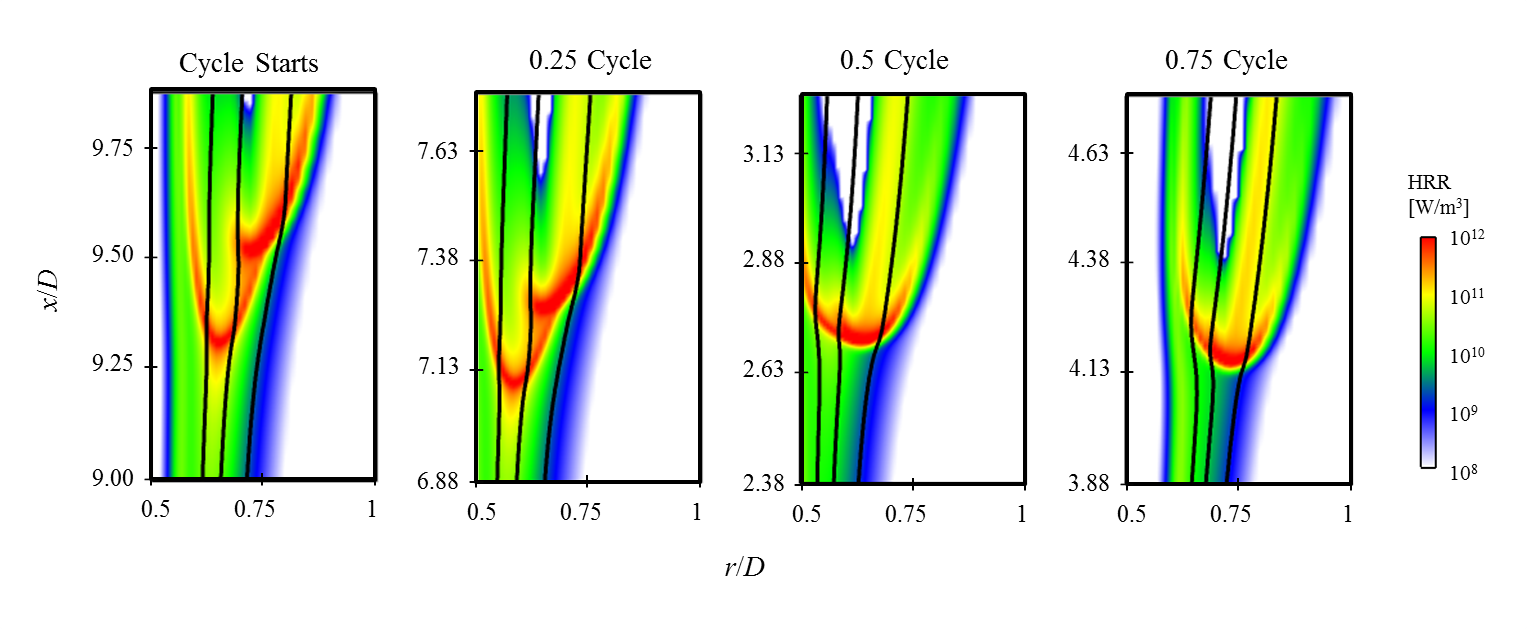
\includegraphics[trim=6.5mm 7.5mm 7mm 8mm, clip=true, width=0.8\textwidth]{HRR_100Hz.png}
  \normalsize
  \vspace{-0.2in}
  \caption{Heat release rate [W/m$^3$] profile evolution during one oscillation cycle at $100$ Hz.  The iso-contours of $Z_{\rm st} = 0.1$, $Z = 0.2$, and $Z = 0.3$ are outlined from right to left in solid lines, respectively.}
  \label{fig:HRR_100Hz}
\end{figure*}

\subsection{Differentiation of combustion mode}

A density-weighted displacement speed, $S_d$, is often used to distinguish between deflagrations and spontaneous ignition fronts in HCCI combustion~\cite{yoo13}, which is defined from an iso-line of species $k$ as~\cite{ruetsch95,im99}:
\begin{equation*}
S_d = \frac{1}{\rho{_u} |\nabla Y_k|} \left(\dot{\omega}{_k} - \pp{\rho Y_k V_{j,k}}{x_j} \right),
\end{equation*}
where $Y_k$, $V_{j,k}$, and $\dot{\omega}{_k}$ denote species mass fraction, diffusion velocity in the $j$-direction, and net production rate, respectively, and $\rho {_u}$ is the density of the unburnt mixture.  $S_d$ at the leading point is insensitive to the choice of major product species in the current study.  Consequently, H$_2$O was chosen for simplicity.  Both the laminar flame speed $S_L$ and the unburnt mixture density $\rho {_u}$ were obtained from laminar flame speed calculations using the FlameMaster code~\cite{flamemaster}.  The composition and temperature boundary conditions for the laminar flame speed calculations were based on the sampled mixture fraction at the leading point and linearly interpolated, in mixture fraction space, between the corresponding inlet values of the fuel and coflow streams.

The normalized displacement velocities for the steady autoignition front (8.0 m/s) and tribrachial flame (2.4 m/s) are shown in Fig.~\ref{fig:sd_hys} as the top and bottom solid circles, respectively.  The $S_d/S_L$ for the steady tribrachial flame is around unity, while this value is around eight for the autoignition front.  These values are similar to those in HCCI combustion studies~\cite{yoo13} and therefore can be used to benchmark the unsteady cases.  The profile of $S_d/S_L$ is bounded by but does not fully reach the two steady values, indicating that, while the chemical structure responds to the flow dynamics, such response is not fast enough to reach steady-state.

Given the same inlet velocity, the reacting fronts have different displacement velocities during the cycle of decreasing- and increasing-velocity, demonstrating a hysteric behavior.  The shift in the displacement velocity indicates different dominant chemical reactions, and analysis of the dominant chemical reactions will reveal the mechanism of the hysteresis.

\begin{figure}[t]
  \centering
  \scriptsize
  \resizebox{0.5\textwidth}{!}{% GNUPLOT: LaTeX picture with Postscript
\begingroup
  \makeatletter
  \providecommand\color[2][]{%
    \GenericError{(gnuplot) \space\space\space\@spaces}{%
      Package color not loaded in conjunction with
      terminal option `colourtext'%
    }{See the gnuplot documentation for explanation.%
    }{Either use 'blacktext' in gnuplot or load the package
      color.sty in LaTeX.}%
    \renewcommand\color[2][]{}%
  }%
  \providecommand\includegraphics[2][]{%
    \GenericError{(gnuplot) \space\space\space\@spaces}{%
      Package graphicx or graphics not loaded%
    }{See the gnuplot documentation for explanation.%
    }{The gnuplot epslatex terminal needs graphicx.sty or graphics.sty.}%
    \renewcommand\includegraphics[2][]{}%
  }%
  \providecommand\rotatebox[2]{#2}%
  \@ifundefined{ifGPcolor}{%
    \newif\ifGPcolor
    \GPcolortrue
  }{}%
  \@ifundefined{ifGPblacktext}{%
    \newif\ifGPblacktext
    \GPblacktexttrue
  }{}%
  % define a \g@addto@macro without @ in the name:
  \let\gplgaddtomacro\g@addto@macro
  % define empty templates for all commands taking text:
  \gdef\gplbacktext{}%
  \gdef\gplfronttext{}%
  \makeatother
  \ifGPblacktext
    % no textcolor at all
    \def\colorrgb#1{}%
    \def\colorgray#1{}%
  \else
    % gray or color?
    \ifGPcolor
      \def\colorrgb#1{\color[rgb]{#1}}%
      \def\colorgray#1{\color[gray]{#1}}%
      \expandafter\def\csname LTw\endcsname{\color{white}}%
      \expandafter\def\csname LTb\endcsname{\color{black}}%
      \expandafter\def\csname LTa\endcsname{\color{black}}%
      \expandafter\def\csname LT0\endcsname{\color[rgb]{1,0,0}}%
      \expandafter\def\csname LT1\endcsname{\color[rgb]{0,1,0}}%
      \expandafter\def\csname LT2\endcsname{\color[rgb]{0,0,1}}%
      \expandafter\def\csname LT3\endcsname{\color[rgb]{1,0,1}}%
      \expandafter\def\csname LT4\endcsname{\color[rgb]{0,1,1}}%
      \expandafter\def\csname LT5\endcsname{\color[rgb]{1,1,0}}%
      \expandafter\def\csname LT6\endcsname{\color[rgb]{0,0,0}}%
      \expandafter\def\csname LT7\endcsname{\color[rgb]{1,0.3,0}}%
      \expandafter\def\csname LT8\endcsname{\color[rgb]{0.5,0.5,0.5}}%
    \else
      % gray
      \def\colorrgb#1{\color{black}}%
      \def\colorgray#1{\color[gray]{#1}}%
      \expandafter\def\csname LTw\endcsname{\color{white}}%
      \expandafter\def\csname LTb\endcsname{\color{black}}%
      \expandafter\def\csname LTa\endcsname{\color{black}}%
      \expandafter\def\csname LT0\endcsname{\color{black}}%
      \expandafter\def\csname LT1\endcsname{\color{black}}%
      \expandafter\def\csname LT2\endcsname{\color{black}}%
      \expandafter\def\csname LT3\endcsname{\color{black}}%
      \expandafter\def\csname LT4\endcsname{\color{black}}%
      \expandafter\def\csname LT5\endcsname{\color{black}}%
      \expandafter\def\csname LT6\endcsname{\color{black}}%
      \expandafter\def\csname LT7\endcsname{\color{black}}%
      \expandafter\def\csname LT8\endcsname{\color{black}}%
    \fi
  \fi
  \setlength{\unitlength}{0.0500bp}%
  \begin{picture}(5760.00,4032.00)%
    \gplgaddtomacro\gplbacktext{%
      \csname LTb\endcsname%
      \put(588,704){\makebox(0,0)[r]{\strut{} 0}}%
      \put(588,1317){\makebox(0,0)[r]{\strut{} 2}}%
      \put(588,1929){\makebox(0,0)[r]{\strut{} 4}}%
      \put(588,2542){\makebox(0,0)[r]{\strut{} 6}}%
      \put(588,3154){\makebox(0,0)[r]{\strut{} 8}}%
      \put(588,3767){\makebox(0,0)[r]{\strut{} 10}}%
      \put(720,484){\makebox(0,0){\strut{} 0}}%
      \put(1584,484){\makebox(0,0){\strut{} 2}}%
      \put(2448,484){\makebox(0,0){\strut{} 4}}%
      \put(3311,484){\makebox(0,0){\strut{} 6}}%
      \put(4175,484){\makebox(0,0){\strut{} 8}}%
      \put(5039,484){\makebox(0,0){\strut{} 10}}%
      \put(-50,2235){\rotatebox{-270}{\makebox(0,0){\strut{}\vspace{-28pt}$S_d/S_L$}}}%
      \put(2879,154){\makebox(0,0){\strut{}$U_{\rm inlet}$}}%
      \put(936,2695){\makebox(0,0)[l]{\strut{}Decreasing-velocity}}%
      \put(3527,1163){\makebox(0,0)[l]{\strut{}Increasing-velocity}}%
    }%
    \gplgaddtomacro\gplfronttext{%
      \csname LTb\endcsname%
      \put(1377,3618){\makebox(0,0)[r]{\strut{}Steady}}%
      \csname LTb\endcsname%
      \put(1377,3442){\makebox(0,0)[r]{\strut{}100 Hz}}%
      \csname LTb\endcsname%
      \put(1377,3266){\makebox(0,0)[r]{\strut{}50 Hz}}%
      \csname LTb\endcsname%
      \put(1377,3090){\makebox(0,0)[r]{\strut{}25 Hz}}%
    }%
    \gplbacktext
    \put(0,0){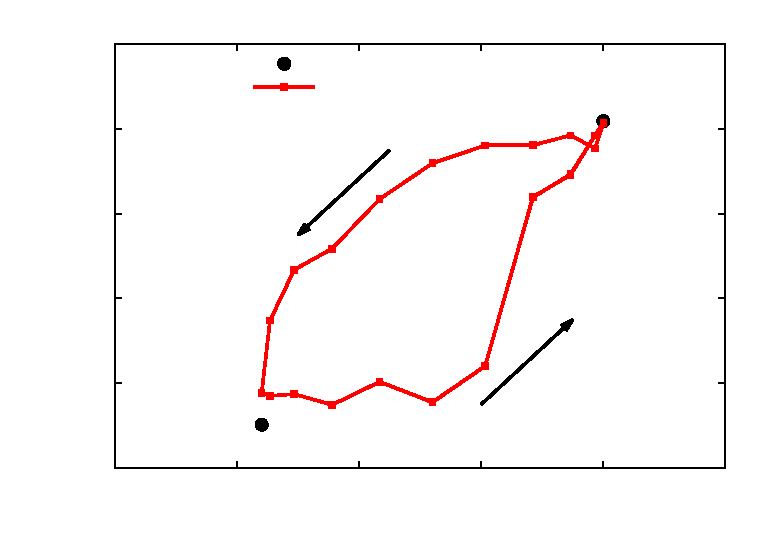
\includegraphics{sd_hys}}%
    \gplfronttext
  \end{picture}%
\endgroup
}
  \normalsize
  \vspace{-0.2in}
  \caption{Normalized displacement velocities at various inlet velocities for steady and unsteady cases.}
  \label{fig:sd_hys}
\end{figure}

 According to the steady case analysis~\cite{deng15b}, the hydrogen peroxide branching reaction (H$_2$O$_2$ + M $\Longleftrightarrow$ OH + OH + M) and the H radical branching reaction (H + O$_2$ $\Longleftrightarrow$ O + OH) are the dominant chain branching reactions at the leading point of the autoignition front and tribrachial flame, respectively.  Due to the longer residence time, hydrogen peroxide accumulation is much higher upstream of the autoignition front compared to the tribrachial flame front.

\begin{figure}[t]
  \centering
  \scriptsize
  \resizebox{0.49\textwidth}{!}{% GNUPLOT: LaTeX picture with Postscript
\begingroup
  \makeatletter
  \providecommand\color[2][]{%
    \GenericError{(gnuplot) \space\space\space\@spaces}{%
      Package color not loaded in conjunction with
      terminal option `colourtext'%
    }{See the gnuplot documentation for explanation.%
    }{Either use 'blacktext' in gnuplot or load the package
      color.sty in LaTeX.}%
    \renewcommand\color[2][]{}%
  }%
  \providecommand\includegraphics[2][]{%
    \GenericError{(gnuplot) \space\space\space\@spaces}{%
      Package graphicx or graphics not loaded%
    }{See the gnuplot documentation for explanation.%
    }{The gnuplot epslatex terminal needs graphicx.sty or graphics.sty.}%
    \renewcommand\includegraphics[2][]{}%
  }%
  \providecommand\rotatebox[2]{#2}%
  \@ifundefined{ifGPcolor}{%
    \newif\ifGPcolor
    \GPcolortrue
  }{}%
  \@ifundefined{ifGPblacktext}{%
    \newif\ifGPblacktext
    \GPblacktexttrue
  }{}%
  % define a \g@addto@macro without @ in the name:
  \let\gplgaddtomacro\g@addto@macro
  % define empty templates for all commands taking text:
  \gdef\gplbacktext{}%
  \gdef\gplfronttext{}%
  \makeatother
  \ifGPblacktext
    % no textcolor at all
    \def\colorrgb#1{}%
    \def\colorgray#1{}%
  \else
    % gray or color?
    \ifGPcolor
      \def\colorrgb#1{\color[rgb]{#1}}%
      \def\colorgray#1{\color[gray]{#1}}%
      \expandafter\def\csname LTw\endcsname{\color{white}}%
      \expandafter\def\csname LTb\endcsname{\color{black}}%
      \expandafter\def\csname LTa\endcsname{\color{black}}%
      \expandafter\def\csname LT0\endcsname{\color[rgb]{1,0,0}}%
      \expandafter\def\csname LT1\endcsname{\color[rgb]{0,1,0}}%
      \expandafter\def\csname LT2\endcsname{\color[rgb]{0,0,1}}%
      \expandafter\def\csname LT3\endcsname{\color[rgb]{1,0,1}}%
      \expandafter\def\csname LT4\endcsname{\color[rgb]{0,1,1}}%
      \expandafter\def\csname LT5\endcsname{\color[rgb]{1,1,0}}%
      \expandafter\def\csname LT6\endcsname{\color[rgb]{0,0,0}}%
      \expandafter\def\csname LT7\endcsname{\color[rgb]{1,0.3,0}}%
      \expandafter\def\csname LT8\endcsname{\color[rgb]{0.5,0.5,0.5}}%
    \else
      % gray
      \def\colorrgb#1{\color{black}}%
      \def\colorgray#1{\color[gray]{#1}}%
      \expandafter\def\csname LTw\endcsname{\color{white}}%
      \expandafter\def\csname LTb\endcsname{\color{black}}%
      \expandafter\def\csname LTa\endcsname{\color{black}}%
      \expandafter\def\csname LT0\endcsname{\color{black}}%
      \expandafter\def\csname LT1\endcsname{\color{black}}%
      \expandafter\def\csname LT2\endcsname{\color{black}}%
      \expandafter\def\csname LT3\endcsname{\color{black}}%
      \expandafter\def\csname LT4\endcsname{\color{black}}%
      \expandafter\def\csname LT5\endcsname{\color{black}}%
      \expandafter\def\csname LT6\endcsname{\color{black}}%
      \expandafter\def\csname LT7\endcsname{\color{black}}%
      \expandafter\def\csname LT8\endcsname{\color{black}}%
    \fi
  \fi
  \setlength{\unitlength}{0.0500bp}%
  \begin{picture}(4320.00,3024.00)%
    \gplgaddtomacro\gplbacktext{%
      \csname LTb\endcsname%
      \put(948,704){\makebox(0,0)[r]{\strut{}0.0e+00}}%
      \put(948,1115){\makebox(0,0)[r]{\strut{}6.0e-03}}%
      \put(948,1526){\makebox(0,0)[r]{\strut{}1.2e-02}}%
      \put(948,1937){\makebox(0,0)[r]{\strut{}1.8e-02}}%
      \put(948,2348){\makebox(0,0)[r]{\strut{}2.4e-02}}%
      \put(948,2759){\makebox(0,0)[r]{\strut{}3.0e-02}}%
      \put(1080,484){\makebox(0,0){\strut{} 0}}%
      \put(1649,484){\makebox(0,0){\strut{} 2}}%
      \put(2217,484){\makebox(0,0){\strut{} 4}}%
      \put(2786,484){\makebox(0,0){\strut{} 6}}%
      \put(3354,484){\makebox(0,0){\strut{} 8}}%
      \put(3923,484){\makebox(0,0){\strut{} 10}}%
      \put(-218,1731){\rotatebox{-270}{\makebox(0,0){\strut{}\vspace{-28pt}$Y_{\rm H_2O_2}$}}}%
      \put(2501,154){\makebox(0,0){\strut{}$x/D$}}%
    }%
    \gplgaddtomacro\gplfronttext{%
      \csname LTb\endcsname%
      \put(2763,2603){\makebox(0,0)[r]{\strut{}Steady 2.4 m/s}}%
      \csname LTb\endcsname%
      \put(2763,2427){\makebox(0,0)[r]{\strut{}Steady 8.0 m/s}}%
      \csname LTb\endcsname%
      \put(2763,2251){\makebox(0,0)[r]{\strut{}0.25 cycle}}%
      \csname LTb\endcsname%
      \put(2763,2075){\makebox(0,0)[r]{\strut{}0.45 cycle}}%
      \csname LTb\endcsname%
      \put(2763,1899){\makebox(0,0)[r]{\strut{}0.5 cycle}}%
    }%
    \gplbacktext
    \put(0,0){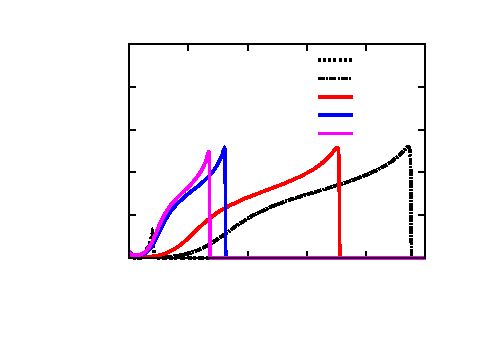
\includegraphics{H2O2_up}}%
    \gplfronttext
  \end{picture}%
\endgroup
}
  \resizebox{0.49\textwidth}{!}{% GNUPLOT: LaTeX picture with Postscript
\begingroup
  \makeatletter
  \providecommand\color[2][]{%
    \GenericError{(gnuplot) \space\space\space\@spaces}{%
      Package color not loaded in conjunction with
      terminal option `colourtext'%
    }{See the gnuplot documentation for explanation.%
    }{Either use 'blacktext' in gnuplot or load the package
      color.sty in LaTeX.}%
    \renewcommand\color[2][]{}%
  }%
  \providecommand\includegraphics[2][]{%
    \GenericError{(gnuplot) \space\space\space\@spaces}{%
      Package graphicx or graphics not loaded%
    }{See the gnuplot documentation for explanation.%
    }{The gnuplot epslatex terminal needs graphicx.sty or graphics.sty.}%
    \renewcommand\includegraphics[2][]{}%
  }%
  \providecommand\rotatebox[2]{#2}%
  \@ifundefined{ifGPcolor}{%
    \newif\ifGPcolor
    \GPcolortrue
  }{}%
  \@ifundefined{ifGPblacktext}{%
    \newif\ifGPblacktext
    \GPblacktexttrue
  }{}%
  % define a \g@addto@macro without @ in the name:
  \let\gplgaddtomacro\g@addto@macro
  % define empty templates for all commands taking text:
  \gdef\gplbacktext{}%
  \gdef\gplfronttext{}%
  \makeatother
  \ifGPblacktext
    % no textcolor at all
    \def\colorrgb#1{}%
    \def\colorgray#1{}%
  \else
    % gray or color?
    \ifGPcolor
      \def\colorrgb#1{\color[rgb]{#1}}%
      \def\colorgray#1{\color[gray]{#1}}%
      \expandafter\def\csname LTw\endcsname{\color{white}}%
      \expandafter\def\csname LTb\endcsname{\color{black}}%
      \expandafter\def\csname LTa\endcsname{\color{black}}%
      \expandafter\def\csname LT0\endcsname{\color[rgb]{1,0,0}}%
      \expandafter\def\csname LT1\endcsname{\color[rgb]{0,1,0}}%
      \expandafter\def\csname LT2\endcsname{\color[rgb]{0,0,1}}%
      \expandafter\def\csname LT3\endcsname{\color[rgb]{1,0,1}}%
      \expandafter\def\csname LT4\endcsname{\color[rgb]{0,1,1}}%
      \expandafter\def\csname LT5\endcsname{\color[rgb]{1,1,0}}%
      \expandafter\def\csname LT6\endcsname{\color[rgb]{0,0,0}}%
      \expandafter\def\csname LT7\endcsname{\color[rgb]{1,0.3,0}}%
      \expandafter\def\csname LT8\endcsname{\color[rgb]{0.5,0.5,0.5}}%
    \else
      % gray
      \def\colorrgb#1{\color{black}}%
      \def\colorgray#1{\color[gray]{#1}}%
      \expandafter\def\csname LTw\endcsname{\color{white}}%
      \expandafter\def\csname LTb\endcsname{\color{black}}%
      \expandafter\def\csname LTa\endcsname{\color{black}}%
      \expandafter\def\csname LT0\endcsname{\color{black}}%
      \expandafter\def\csname LT1\endcsname{\color{black}}%
      \expandafter\def\csname LT2\endcsname{\color{black}}%
      \expandafter\def\csname LT3\endcsname{\color{black}}%
      \expandafter\def\csname LT4\endcsname{\color{black}}%
      \expandafter\def\csname LT5\endcsname{\color{black}}%
      \expandafter\def\csname LT6\endcsname{\color{black}}%
      \expandafter\def\csname LT7\endcsname{\color{black}}%
      \expandafter\def\csname LT8\endcsname{\color{black}}%
    \fi
  \fi
  \setlength{\unitlength}{0.0500bp}%
  \begin{picture}(4320.00,3024.00)%
    \gplgaddtomacro\gplbacktext{%
      \csname LTb\endcsname%
      \put(948,704){\makebox(0,0)[r]{\strut{}0.0e+00}}%
      \put(948,1115){\makebox(0,0)[r]{\strut{}6.0e-03}}%
      \put(948,1526){\makebox(0,0)[r]{\strut{}1.2e-02}}%
      \put(948,1937){\makebox(0,0)[r]{\strut{}1.8e-02}}%
      \put(948,2348){\makebox(0,0)[r]{\strut{}2.4e-02}}%
      \put(948,2759){\makebox(0,0)[r]{\strut{}3.0e-02}}%
      \put(1080,484){\makebox(0,0){\strut{} 0}}%
      \put(1649,484){\makebox(0,0){\strut{} 2}}%
      \put(2217,484){\makebox(0,0){\strut{} 4}}%
      \put(2786,484){\makebox(0,0){\strut{} 6}}%
      \put(3354,484){\makebox(0,0){\strut{} 8}}%
      \put(3923,484){\makebox(0,0){\strut{} 10}}%
      \put(-218,1731){\rotatebox{-270}{\makebox(0,0){\strut{}\vspace{-28pt}$Y_{\rm H_2O_2}$}}}%
      \put(2501,154){\makebox(0,0){\strut{}$x/D$}}%
    }%
    \gplgaddtomacro\gplfronttext{%
      \csname LTb\endcsname%
      \put(2479,2603){\makebox(0,0)[r]{\strut{}Steady 2.4 m/s}}%
      \csname LTb\endcsname%
      \put(2479,2427){\makebox(0,0)[r]{\strut{}Steady 8.0 m/s}}%
      \csname LTb\endcsname%
      \put(2479,2251){\makebox(0,0)[r]{\strut{}0.5 cycle}}%
      \csname LTb\endcsname%
      \put(2479,2075){\makebox(0,0)[r]{\strut{}0.55 cycle}}%
      \csname LTb\endcsname%
      \put(2479,1899){\makebox(0,0)[r]{\strut{}0.65 cycle}}%
      \csname LTb\endcsname%
      \put(2479,1723){\makebox(0,0)[r]{\strut{}0.75 cycle}}%
      \csname LTb\endcsname%
      \put(2479,1547){\makebox(0,0)[r]{\strut{}0.85 cycle}}%
    }%
    \gplbacktext
    \put(0,0){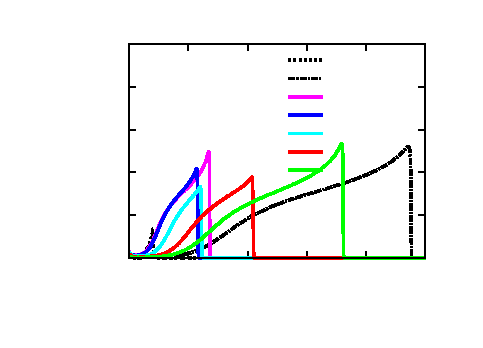
\includegraphics{H2O2_down}}%
    \gplfronttext
  \end{picture}%
\endgroup
}
  \vspace{-0.2in}
  \normalsize
  \caption{The comparison of hydrogen peroxide mass fraction profiles along the $Z = 0.24$ iso-contour at steady state and at $100$ Hz during the decreasing-velocity cycle (left) and increasing-velocity cycle (right).}
  \label{fig:H2O2_updown}
\end{figure}

As hydrogen peroxide plays different roles in the tribrachial flame and autoignition front, its spatial profiles along the $Z = 0.24$ iso-contour are compared in Fig.~\ref{fig:H2O2_updown}.  Hydrogen peroxide continues accumulating until either autoignition occurs or it is consumed at the flame front, resulting in a sharp drop in its mass fraction.  However, the peak value of the hydrogen peroxide mass fraction differs by a factor of five between a steady autoignition front and tribrachial flame, which implies its different significance in these two combustion modes and sets the benchmark for the unsteady evolution.  As the inlet velocity decreases from $8.0$ m/s, the peak $Y_{\rm H{_2}O{_2}}$ almost remains constant, indicating that the chemical structure is very close to the steady autoignition case.  Consequently, the dominant chemical pathway remains as H$_2$O$_2$ + M $\Longleftrightarrow$ OH + OH + M, and autoignition is the dominant combustion process, resulting in large $S_d/S_L$.  However, as the flow velocity decreases, a larger gradient is achieved, resulting in steeper profiles and smaller $S_d/S_L$, according to the definition of the displacement velocity.

Even when the inlet velocity reaches the minimum $2.4$ m/s, the reacting front continues to move upstream.  Inlet velocity changes slowest around the half cycle, allowing the chemical structure to respond to the hydrodynamic changes.  As shown on the right of Fig.~\ref{fig:H2O2_updown}, the peak $Y_{\rm H{_2}O{_2}}$ decreases from $0.5$ to $0.65$ of the cycle.  At this stage, autoignition is not fully activated, since the peak $Y_{\rm H{_2}O{_2}}$ is lower than the steady autoignition case.  However, the peak $Y_{\rm H{_2}O{_2}}$ is still larger than the steady tribrachial flame.  Therefore, the $S_d/S_L$ of the tribrachial structure is close to but slightly larger than a steady tribrachial flame, for it is propagating into a partially reacted mixture.

This tribrachial structure is convected downstream, as inlet velocity further increases from $0.65$ to $0.75$ of the cycle.  The unburnt mixture upstream of the flame accumulates radicals and heat as it moves downstream.  Due to finite ignition delay time, $S_d/S_L$ almost keeps constant during the induction period, and hence shows a flat bottom in Fig.~\ref{fig:sd_hys}, before autoignition finally occurs, indicated by a sudden jump of $S_d/S_L$.

\section{Conclusion}

Axisymmetric laminar nonpremixed DME coflow flames at elevated temperatures and pressures with sinusoidally oscillating inlet velocities were computationally investigated.  The inlet velocity oscillates between $2.4$ and $8.0$ m/s at $100$ Hz.  Flame dynamics in such oscillating flows and frequency effects on the hydrodynamics-chemistry coupling were analyzed.

The heat release rate profiles were examined to describe the thermal structure.  The morphology of the thermal structure transitions between tribrachial and multibrachial.  The multibrachial structure is favored when the inlet velocity is higher, although there is hysteresis during the transition.  Such structures agree well with the steady cases in Deng~\emph{et al.}~\cite{deng15b}, which correspond to different combustion modes: tribrachial flame and autoignition.  Normalized displacement velocity was defined to differentiate these two modes in the current study and compare with the steady cases.

According to the steady results, the normalized displacement velocity for a tribrachial flame is around unity and is larger for autoignition.  The same criterion was applied to the unsteady cases to elucidate the evolution of combustion mode.  As the inlet velocity decreases, autoignition is the dominant combustion process until flame chemistry takes over around the most upstream location and slowest inlet velocity.  The tribrachial flame is convected downstream as the flow velocity increases.  The radical and heat accumulation upstream of the tribrachial flame finally results in autoignition, showing a sudden increase in the normalized displacement velocity.  The finite ignition delay time results in the hysteretic behavior during the evolution of combustion mode.

\section*{Acknowledgments}

This research was supported in part by the Air Force Office of Scientific Research (AFOSR) under the technical management of Dr. Mitat Birkan.

\bibliographystyle{essci}
\bibliography{ESS_uns}


\end{document}
